\documentclass[a4paper]{article}
\usepackage[T1]{fontenc}
\usepackage{graphicx}
\graphicspath{ {./img/} }
\usepackage{ragged2e}
\title{Projektowanie i programowanie gier \\
\vspace{5px}
\large Sprawozdanie z części laboratoryjnej }
\date{semestr letni 2023/2024}

  \author{
    \centering
    \begin{tabular}{c}
      Eryk Mika 264451  \\[2ex]
      Prowadzący: Szymon Datko
    \end{tabular}
  }

\begin{document}
\maketitle
\renewcommand{\figurename}{Zrzut}
\begin{sloppypar}
	\section{Wstęp}
	\justifying
	Celem laboratoriów było zapoznanie się z wybranym silnikiem graficznym - Godot. W tym celu zrealizowałem 2 tutoriale:
	\begin{itemize}
		\item Your first 2D game - tutorial z oficjalnej strony Godot Engine
		\item Godot: Creating a Simple 3D Game - seria filmów na YouTubie.
	\end{itemize}
	Oba tutoriale zaznajamiają czytelnika z podstawowymi funkcjonalnościami środowiwska Godot. Efektem końcowym pracy wynikającej
	z zrealizowania każdej ze ścieżek było wykonanie przeze mnie prostej gry - odpowiednio 2D oraz 3D z uwzględnieniem takich
	aspektów jak logika (oprogramowana za pomocą GDScript - języka podobnego do języka Python), grafika (sprite-y, modele 3D),
	obsługa kontroli zdarzeń w grze za pomocą myszy/klawiatury, efekty dźwiękowe. Cała praca została przeze mnie wykonana przy
	użyciu Godot Engine 4.2.1 na urządzeniu z systemem operacyjnym Ubuntu 22.04 LTS.
	\section{Moja "pierwsza" gra 2D}
	Stworzenie przeze mnie gry w ramach tutorialu składało się z kroków, na które podzielony jest tutorial na stronie; najpierw
	wstępnie skonfigurowałem projekt, utworzyłem scenę gracza (\emph{Player}), za pomocą kodu w języku GDScript wprowadziłem
	logikę dla gracza. Podobne kroki powtórzyłem dla przeciwnika (\emph{Enemy}). Na końcu połączyłem całość w scenę \emph{main},
	dodałem nakładki HUD (\emph{ang. Heads Up Display}) - w tym ilość punktów, przycisk startu gry. Efektem końcowym była trywialna gra,
	w której gracz przemieszcza postać na planszy 2D unikając przeciwników pojawiających się w losowych punktach planszy.
	Poprzez przerobienie tutorialu dowiedziałem się, jak łączy się komponenty takiego projektu w całość, przynajmniej na przykładzie małoskalowej gry.
	Zwróciłem uwagę na sposób przekazywania informacji z jednej sceny do drugiej (emph{signals}) na przykładzie kolizji gracza i przeciwnika.
	\subsection{Zrzuty ekranu z wykonanej pracy}
	Wprowadziłem modyfikacje w stosunku do przykładu przedstawionego w tutorialu - wprowadziłem język polski.
\end{sloppypar}
\begin{center}
	\begin{figure}[htb]
		\centering
		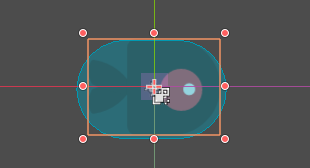
\includegraphics[width=0.6\textwidth]{enemy_collision.png}
		\caption{Określenie granic kolizji dla przeciwnika}
	\end{figure}
	\begin{figure}[htb]
		\centering
		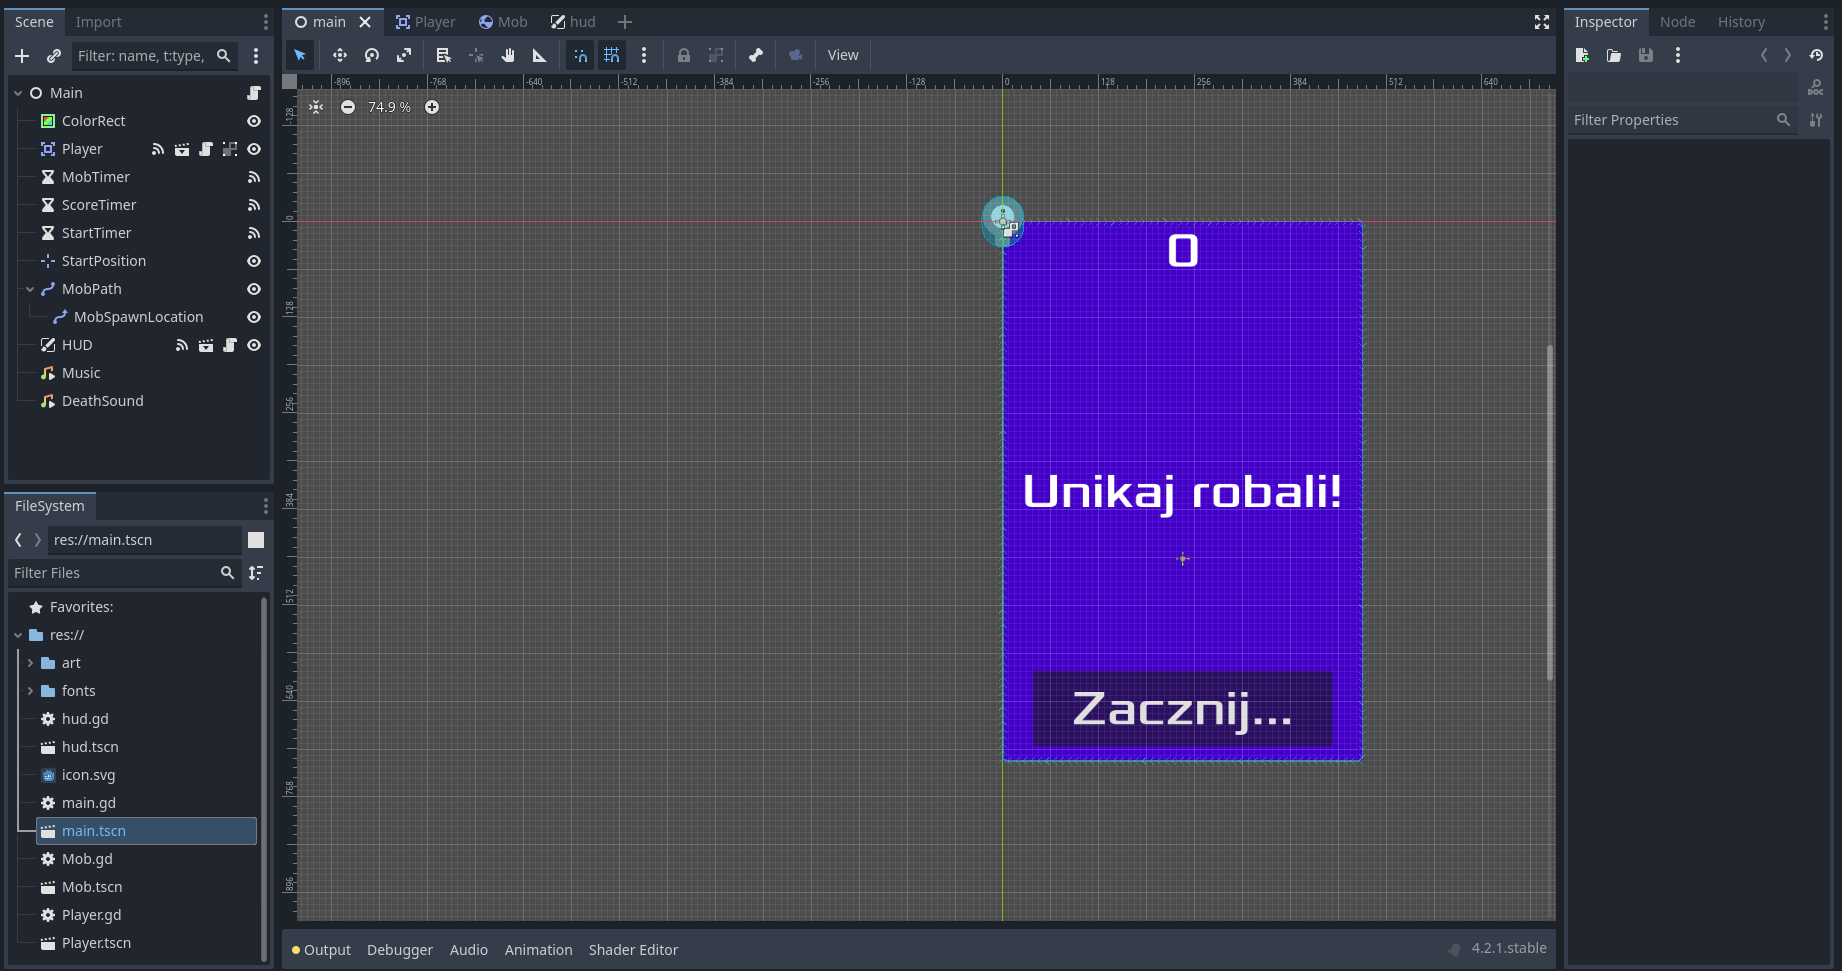
\includegraphics[width=\textwidth]{mob_path.png}
		\caption{Podgląd na główną scenę w edytorze 2D wraz ze ściezką \emph{Enemy}}
	\end{figure}
	\begin{figure}
		\centering
		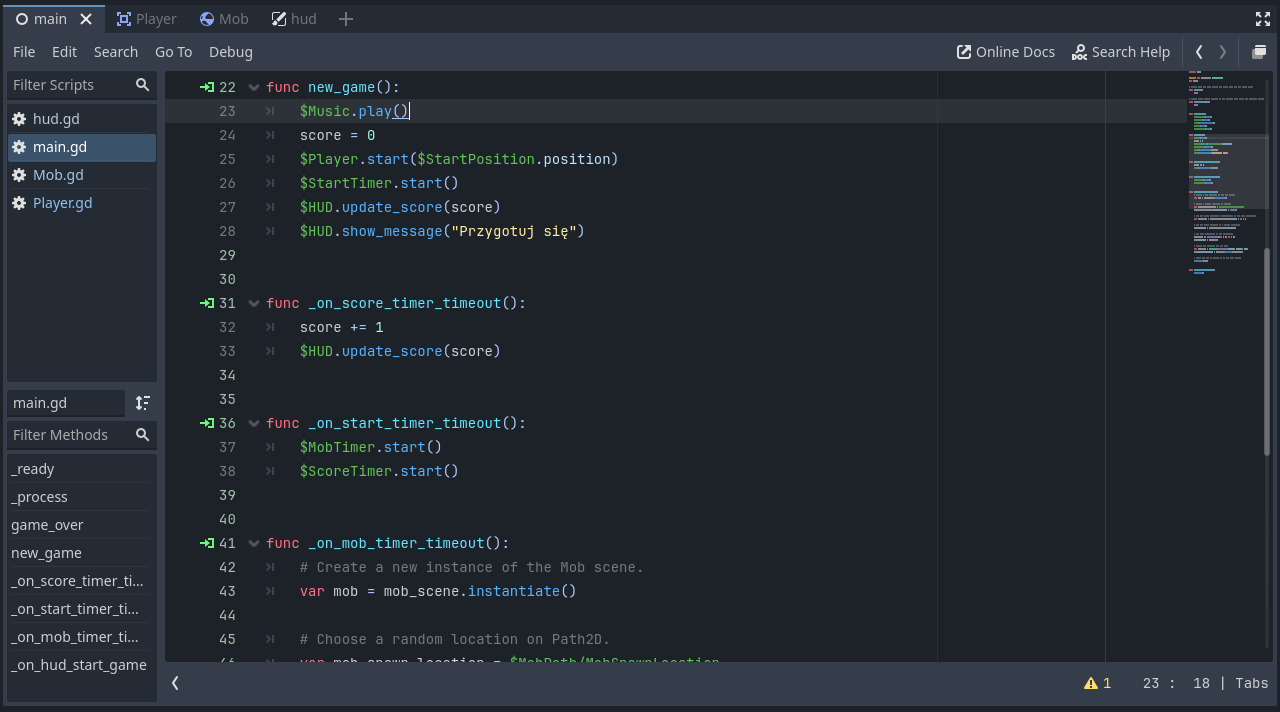
\includegraphics[width=\textwidth]{code.png}
		\caption{Fragment kodu GDScript głównej sceny gry}
	\end{figure}
	\begin{figure}
		\centering
		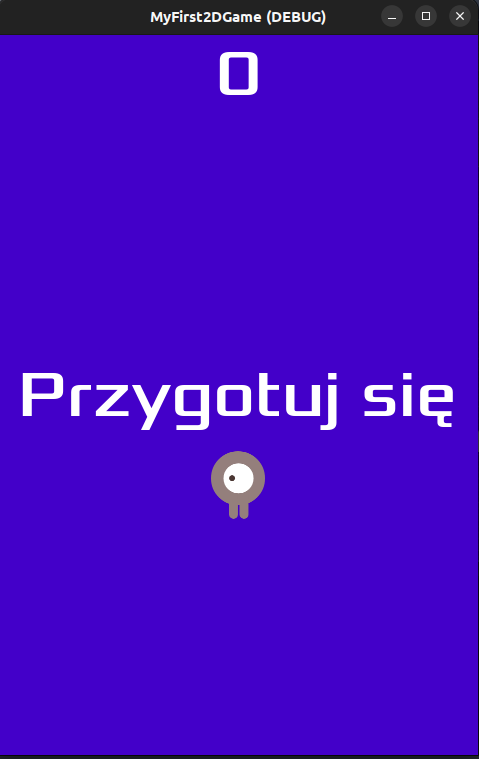
\includegraphics[height=0.35\textheight]{get_ready.png}
		\caption{Ekran rozgrzewający}
	\end{figure}
	\begin{figure}
		\centering
		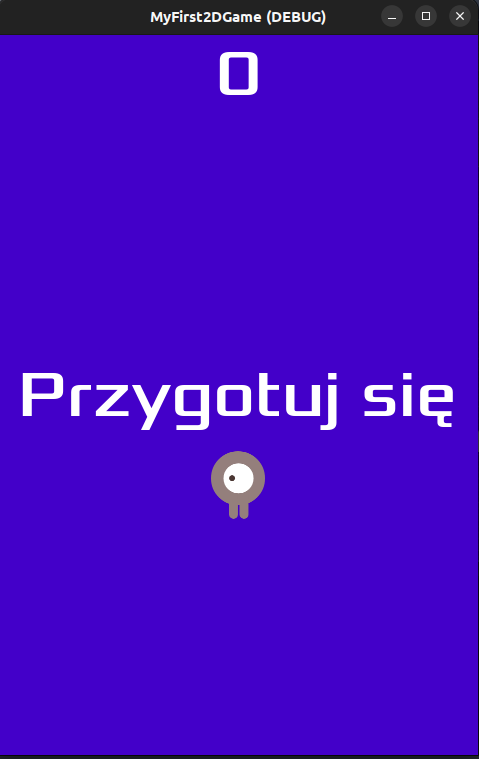
\includegraphics[height=0.35\textheight]{get_ready.png}
		\caption{Ekran rozgrzewający}
	\end{figure}
	\begin{figure}
		\centering
		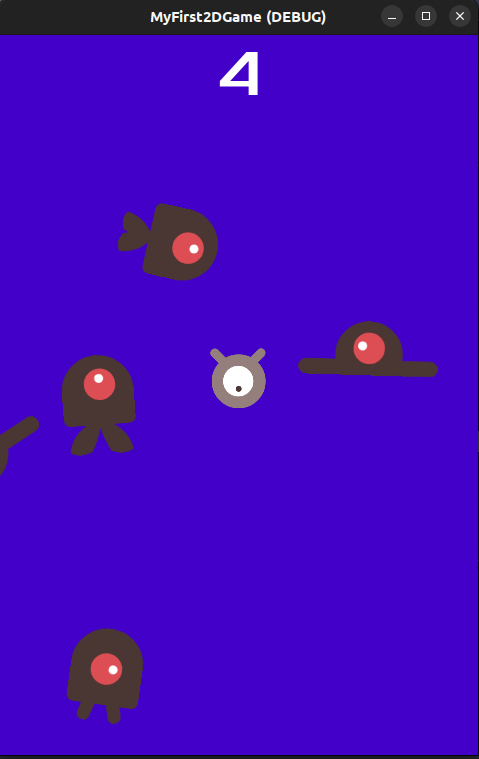
\includegraphics[height=0.35\textheight]{game1.png}
		\caption{W trakcie gry}
	\end{figure}
	\begin{figure}
		\centering
		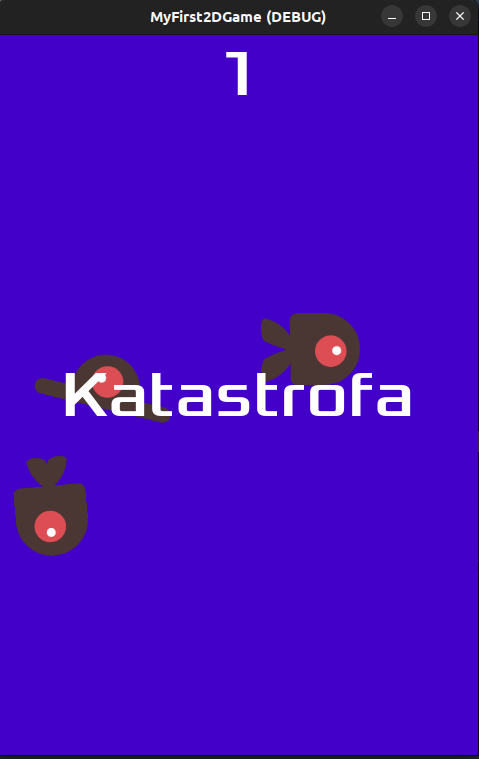
\includegraphics[height=0.35\textheight]{game_over.png}
		\caption{"Game over"}
	\end{figure}
\end{center}
\end{document}
